%%%%%%%%%%%%%%%%%%%%%%%%%%%%%%%%%%%%%%%%%%%%%%%%%%%%%%%%%%%%%%%%%%%%%%%%%%%%%%%%
%2345678901234567890123456789012345678901234567890123456789012345678901234567890
%        1         2         3         4         5         6         7         8
\documentclass[letterpaper, 10 pt, conference]{ieeeconf}  % Comment this line out
                                                          % if you need a4paper
%\documentclass[a4paper, 10pt, conference]{ieeeconf}      % Use this line for a4
                                                          % paper

\IEEEoverridecommandlockouts                              % This command is only
                                                          % needed if you want to
                                                          % use the \thanks command
\overrideIEEEmargins
% See the \addtolength command later in the file to balance the column lengths
% on the last page of the document

\usepackage{epsfig}
\usepackage{amsfonts}
\usepackage{amssymb}
\usepackage{amstext}
\usepackage{amsmath}
\usepackage{xspace}
\usepackage{theorem}
\usepackage{xcolor}
\usepackage{graphicx}
\usepackage{url}
\usepackage{blkarray}
\usepackage{multirow}
\usepackage{tikz}
\usetikzlibrary{calc}
\usepackage{extarrows}
\usetikzlibrary{positioning}
\newcommand{\pincoord}[1]{\tikz[overlay, remember picture] \coordinate (#1);}


\usepackage{xcolor,colortbl}

% The following packages can be found on http:\\www.ctan.org
%\usepackage{graphics} % for pdf, bitmapped graphics files
%\usepackage{epsfig} % for postscript graphics files
%\usepackage{mathptmx} % assumes new font selection scheme installed
%\usepackage{times} % assumes new font selection scheme installed
%\usepackage{amsmath} % assumes amsmath package installed
%\usepackage{amssymb}  % assumes amsmath package installed

\title{\LARGE \bf
Evaluating Dimensionality Reduction Methods
}

\author{Department of Computer Science, Stony Brook University}% stops a space

\begin{document}



\maketitle
\thispagestyle{empty}
\pagestyle{empty}


%%%%%%%%%%%%%%%%%%%%%%%%%%%%%%%%%%%%%%%%%%%%%%%%%%%%%%%%%%%%%%%%%%%%%%%%%%%%%%%%
\begin{abstract}

The dimensionality reduction technique is the process of reducing the number of variables of a highdimensional
dataset, which on reduction preserve the majority of information from the original dataset. In
today’s world, there is an abundant flow of data: from phones, credit cards, home appliances, sensor
equipped buildings, vehicles, big factories and other enormous number of sources. With this data revolution,
the classical statistical analysis as well as making quick decisions based on these data, becomes a new
challenge.The goal is shifted from statistical analysis to new ways of linking datasets with generation of graphical
insights. As the ever-increasing data becomes more and more complex, the curse of dimensionality, which
forbids to reveal hidden insights in low dimension, hinders the businesses as well as new scientific
discoveries. On one hand, the statistical or Machine learning algorithms started to fail due to high variance;
while big data has also introduced processing \& storage barriers. Dimensionality reduction techniques can
sufficiently bring down the higher dimensional data to lower dimensional representations without significant
loss of latent information. In this evaluation, we will try to analyze the inherent problems, suitable reduction
techniques, the challenges and some recent developments in this area.

\end{abstract}
%%%%%%%%%%%%%%%%%%%%%%%%%%%%%%%%%%%%%%%%%%%%%%%%%%%%%%%%%%%%%%%%%%%%%%%%%%%%%%%%
\section{INTRODUCTION}

As the data is increasing, it becomes more difficult to process the real time data as it is incomplete, inconsistent and unorganized. The main challenge is to find the transformation to intrinsic dimension with minimal loss while keeping significance intact. A Dimensionality Reduction technique is the process of reducing the number of variables of a high-dimensional dataset, which on reduction preserve the majority of information from the original dataset. These dimensionality reduction techniques are applied in latent knowledge discovery, feature analysis, machine learning algorithms and visualization. Dimensionality reduction techniques can sufficiently bring down the higher dimensional data to lower dimensional representations without significant loss of latent information. Different comparative studies comparing different dimensionality reduction methods are currently being addressed in the research field. 
In this comparative study, we discuss how we can compare different dimensionality reduction algorithms based on the features like loss of quality and quantitative measures that will help us understand the application and working of each of those algorithms. We have considered the following dimensionality reduction techniques: Principal Component Analysis (PCA), Multidimensional Scaling (MDS), t-Distributed Stochastic Neighbor Embedding(t-SNE), kernel-PCA, IVIS, Uniform Manifold Approximation and Projection(UMAP), and Trimap. Some of the features that we have used to study the above-mentioned techniques include Mapping higher dimensional data into a 2d Mapping grid for visualization, Mantel test, Qualitative measures and quantitative analysis. 


\section{Background Research}

As the data is increasing, it becomes more difficult to process the real time data as it is incomplete,
inconsistent and unorganized. The main challenge is to find the transformation to intrinsic dimension with
minimal loss while keeping significance intact. These dimensionality reduction techniques are applied in
latent knowledge discovery, feature analysis, machine learning algorithms and visualization. Historically,
Linear dimensionality techniques were generally developed in the earlier times, where PCA (Principal
Component Analysis) was among the most popular ones .But, PCA does not work in those cases in
uncorrelated data.

These linear techniques transform the data from high to low dimension via linear combination of variables
(derived variables). But these linear techniques only work when data lies in linear space, which does not cover
the majority of problems which are complex and non-linear. Also, linear dimensionality reduction techniques
are not as capable as non-linear methods to product optimal low-dimensional representations when data
points in the input space are arranged along highly curved surfaces. To overcome these shortcomings of
linear dimensionality reduction methods, non-linear methods were proposed. Among the early invented non-linear methods, MDS and Isomap were popular.

Dimensionality reduction approaches can be divided into feature selection and feature extraction. Feature selection methods try to find a subset of the input attributes. It can be done in the following ways:

\begin{enumerate}
	\item The filter strategy
	\item The wrapper strategy
	\item The embedded strategy
\end{enumerate}

Feature extraction transforms the data in the high dimension space to fewer dimensions where transformation can be linear or non-linear.


\begin{enumerate}
	\item Linear Dimensionality techniques: \\
	Many methods have been proposed that produces compressed data that preserves some features of interest in the data. Some of the linear techniques are :
		\begin{itemize}
			\item PCA (Principal Component Analysis)
			\item LDA (Linear Discriminant Analysis)
		\end{itemize}
	\item Non-Linear Dimensionality techniques: \\
	These can be divided into three categories:
		\begin{enumerate}
			\item Distance preservation:
				\begin{itemize}
					\item MDS (Multidimensional Scaling)
					\item Diffusion Map
					\item Isomap
					\item UMAP (Uniform Manifold Approximation and Projection)
					\item t-SNE (T-distributed Stochastic Neighbour Embedding)
					\item ivis 
					\item TRIMAP
				\end{itemize}
			\item Kernel-based: 
					\begin{itemize}
						\item Kernel PCA
					\end{itemize}
			\item Neural Networks: 
					\begin{itemize}
						\item Autoencoder
					\end{itemize}
		\end{enumerate}
\end{enumerate}


\section{Reduction Techniques}

\subsection{\textbf{UMAP}}
Umap is a novel manifold learning technique for dimensionality reduction. Umap is based on Riemannian
geometry and algebraic topology. Umap is competitive with t-SNE in visualization quality and preserves
more global structure compared to t-SNE. UMAP can be thought of a two-step process. In the first step, a
particular weighted k-neighbor graph is constructed. In the second phase, a low-dimensional layout of the
graph is computed. Umap performs better at preserving global aspects of the high dimensional data as
compared to t-SNE. It uses binary-cross entropy as a cost function instead of the KL divergence used in t-SNE. This leads to a huge change in the global data preservation. UMAP does not use normalization for
high dimensional as well as low dimensional probabilities. Umap somewhat uses the same steps as t-SNE
but with some improvements and absence of normalization.

Properties :
\begin{itemize}
	\item UMAP, unlike t-SNE, does not need pre-dimensionality reduction for converting high-dimensional
data.
	\item UMAP can be used for supervised and semi-supervised reductions.
\end{itemize}

\subsection{\textbf{t-SNE}}
T-distributed Stochastic Neighbor Embedding(t-SNE) is a non-linear dimensionality reduction technique
used to embed high-dimensional data into low dimensions for visualization. t-SNE, uses t-distribution, to
compute similarity between two points. t-SNE works by first constructing the probability distribution for
different pairs of objects in high dimensional data to find points that can be similar. After describing the
probability function for all pairs of high-dimensional objects, t-SNE maps these into lower dimensional space.
It does so by randomly plotting the objects in the lower dimension space, re-computing the probability
function for all pairs of objects and then using the earlier probabilities to group objects in the lowerdimensional
space. t-SNE has over 10 hyper parameters that can be used for optimization. Some of these
include perplexity, number of iterations, learning rate etc.

Properties :
\begin{itemize}
	\item t-SNE works on neighborhood distances and preserve local structure while also revealing presence
of global features like clusters.
	\item t-SNE is usually used to embed high-dimensional data into 2-3 dimensions i.e. for visualization purposes. Thus, it is not assured if t-SNE is going to be useful as a general dimension reduction technique.
	\item t-SNE requires pre-dimensionality reduction before actually applying the algorithm and consumes high memory for its computations.
\end{itemize}

\subsection{AUTOENCODER}
Autoencoder is a data compression algorithm, that, by using neural networks, is able to learn how to compress data into small bits of data and then using that regenerate the original representation of the input. There are two main components of the autoencoder, namely, downsampling and upsampling. These two steps are used together to efficiently obtain the representation of data from which the original representation is reconstructed, without losing much of the data. The down sampling process basically tries to represent the data in the most effective form by extracting the most prominent features from the input\_data. The upsampling step is exactly opposite where in this step the autoencoder tries to read features instead of finding them. It reads features from the compressed data and tries to extract images from them.  

\subsection{IVIS}
Ivis is a machine learning algorithm for reducing dimensionality of very large datasets. It preserves global data structures in a low-dimensional space, adds new data points to existing embeddings using a parametric mapping function, and scales linearly to millions of observations.

\subsection{TRIMAP}
TriMap is a dimensionality reduction technique based on triplet constraints that preserves the global accuracy of the data. The main idea behind TriMap is to capture higher orders of structure with triplet information (instead of pairwise information used by t-SNE and LargeVis), and to minimize a robust loss function for satisfying the chosen triplets. Tri-Map is fast and provides comparable runtime on large datasets.

\vspace{3mm}
\section{DATASETS}
\subsection{MNIST}
The MNIST dataset of database of handwritten digits, published by LeCun, which consists of a training set of labelled 60,000 examples with 10,000 test data. Each of the image in the dataset is of shape of 28x28 and grayscale colorspace with 10 labels representing digits from 0-9.
\vspace{1mm}
\\Example:
\begin{figure}[h!]
	\centering
	
\includegraphics[width=0.94\linewidth]{DATA1.png}
	\label{fig:DATA1.png}
\end{figure}

\subsection{Fashion-MNIST}
The Fashion-MNIST is a dataset consisting of 60,000 training & 10,000 test examples published by Zalando Research. Each of the image in the dataset is a 28x28 grayscale image with associated label from 10 classes.
\vspace{1mm}
\\Example:
\begin{figure}[h!]
	\centering
	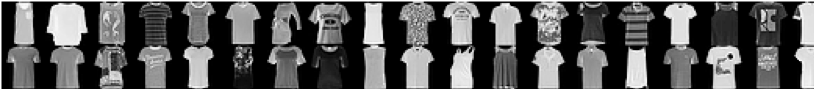
\includegraphics[width=0.94\linewidth]{data2.png}
	\label{fig:data2.png}
\end{figure}

\subsection{COIL-20}
Columbia Object Image Library is a database of 1440 images, which contains grayscale images of 20 objects, rotated in 360 degrees presenting different poses. 
\vspace{1mm}
\\Example:
\begin{figure}[h!]
	\centering
	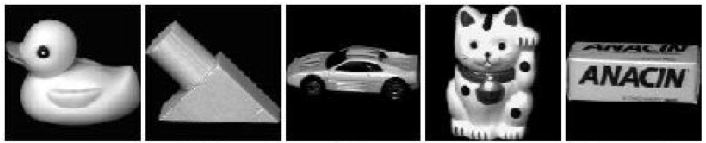
\includegraphics[width=0.94\linewidth]{data3.png}
	\label{fig:data3.png}
\end{figure}

\subsection{CIFAR-10}
A dataset consisting of 60000 32*32 color images of 10 different classes. There are 10 categories present of everyday objects like airplanes, dogs etc.
\vspace{1mm}
\\Example:
\begin{figure}[h!]
	\centering
	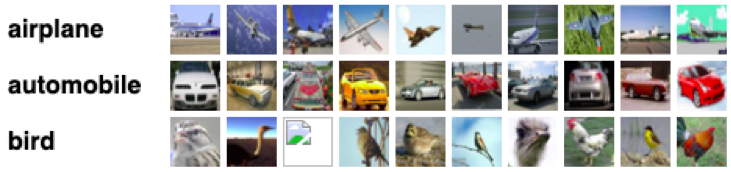
\includegraphics[width=0.94\linewidth]{data4.png}
	\label{fig:data4.png}
\end{figure}

\section{Quantitative Analysis}
There are many different quality assessment measures for evaluating the performance of the DR algorithms. Most of the measures are used to evaluate the local-neighborhood-preservation or the overall- structure-holding performance(global) of the DR methods. Some of the local and global approaches are listed in the table.

\subsection{Distance Preservation}
Historically Distance preservation has been the first and most important criterion used to achieve a DR in a non-linear way. In an ideal scenario, conservation of pairwise distances between different vectors of a dataset ensures that the low dimensional embedding inherits the main geometric properties of the data, such as the overall shape. However, in case of non-linear DR methods, distances are not perfectly preserved. In short, different DR algorithms preserve different types of distances when it comes to dimensionality reduction. These can be pairwise distances, local structural distances and global structures distances etc. E.g. Of these are Kernel PCA, Isomap etc.

\subsection{Topology Preservation}
In the case of topology, the overall shape of the manifold is preserved ie the structural properties of the dataset. These techniques, that can preserve topological characteristics of the input data are also known as local preservation approach. A lattice is defined as a discrete representation of the topology. Most of the DR methods fall into two categories, one in which uses a predefined lattice, e.g. Self-Organizing Maps(SOM’s) and Generative Topographic mapping, and the other one uses a data-driven lattice. The data-driven lattice allows the DR method to change the shape of the lattice or entirely build the lattice while the models are running. E.g of these are Locally Linear Embedding and Laplacian eigenmaps etc.
\begin{figure}[h!]
	\centering
	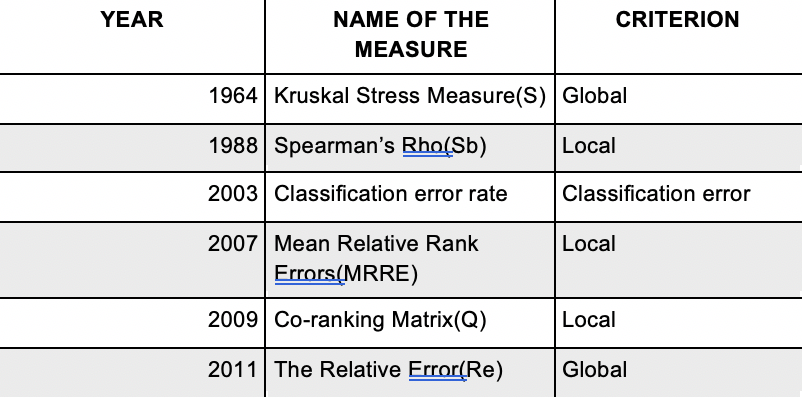
\includegraphics[width=0.94\linewidth]{table.png}
	\label{fig:table.png}
	\caption{Methods for evaluating the quality of DR algorithms}
\end{figure}

\\The degree of correspondence between the distances among points implied by MDS and the matrix input by the user is measured by a stress function called "Kruskal Stress".
\vspace{2mm}

\\\textbf{Spearman's Rho} Siegel and Castellan presented one of the first measures to estimate the topology preservation (TP). This measure estimates the correlation of rank order data. That is, it tries to assess how well the corresponding projection preserves the order of pairwise distances between data-points in high- dimensional space.
\vspace{2mm}

\\\textbf{Mean Relative Rank Errors} Lee and Verleysen developed a quality assessment measure, the mean relative rank errors (MRRE). It is based on ranks of pairwise Euclidean distances within local neighborhoods.
\vspace{2mm}

\\Many different concepts and quality criteria for DR can be summarized using the Co-ranking matrix framework (Q), Several of the aforementioned methods (based on distance ranking in local neighborhoods like MRRE), are easily unified into an overall framework.

\vspace{4mm}

\section[Visualization]{Visualization 2D Plots}
Fig 2 shows the 2D representations of different datasets using various dimensionality reduction methods.
\begin{figure}[h!]
	\centering
	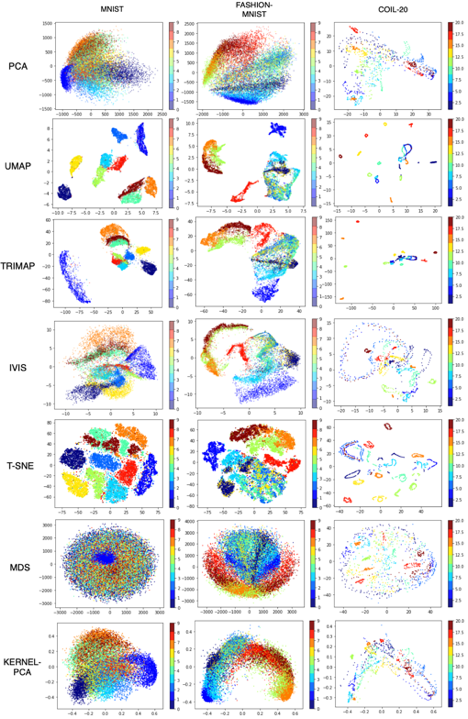
\includegraphics[width=0.94\linewidth]{screenshot001.png}
	\label{fig:screenshot001}
	\caption{2D representations}
\end{figure}

\section{Quantitative Analysis}
According to the Nature Paper, to analyze qualitatively, Author have formulated various methodologies to formalize the qualitative analysis. Following the same path, we also used similar methods. First, on the computational aspects of the running time of the reduction algorithms, we benchmarked all of our five datasets by time taken to complete the data reduction. Second, to assess the ability of each reduction algorithm to separate the datasets into defined 2D reduced embeddings, we trained a Random Forest classifier on the reduced dataset. Third, we analyzed each of seven dimensionality reduction algorithms on the basis of how each algorithm really have the capability to preserve the global structure by comparison of distances between all pairwise distances of high-dimension and reduced dimension with the help of Mantel test.

\\Let’s dive into more detailed analysis below.
\\Comparing time taken by different algorithms
\begin{figure}[h!]
	\centering
	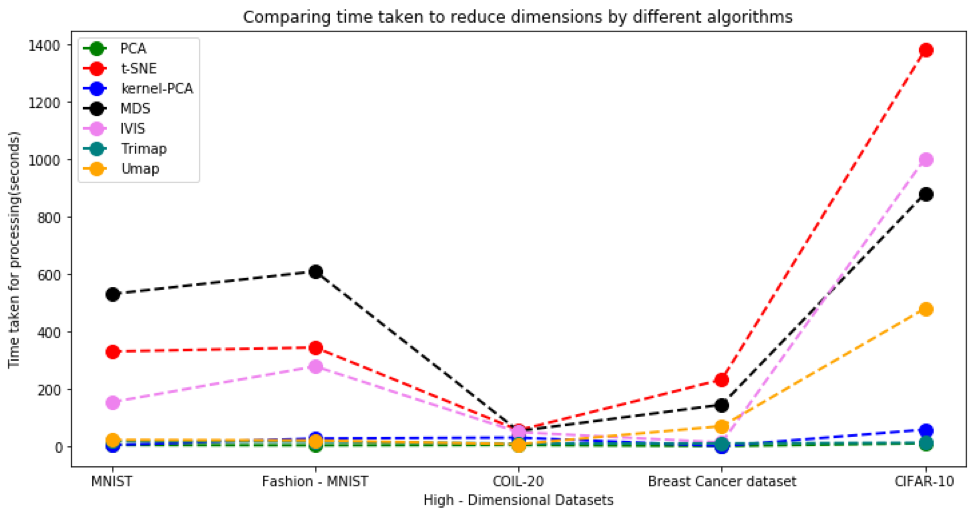
\includegraphics[width=0.94\linewidth]{qual1.png}
	\label{fig:qual1}
	\caption{Comparing time taken to reduce dimensions by different algorithms}
\end{figure}
\vspace{3mm}
\\\textbf{Observations:}
The above plot gives a qualitative comparison on the time taken by different methods to fit a high-dimensional dataset. We applied 7 DR methods on the available datasets and compared the execution time for each method versus the others. As we can see clearly, MDS is usually slower than other algorithms. Even t-SNE is generally slower compared to other algorithms. This maybe because it does not have the scaling properties. Also, one of the fastest algorithms is the PCA, it usually takes the least amount of time to execute. Algorithms like Trimap, IVIS and kernel-PCA take average time in terms of execution. To gain a deeper insight and get more accurate comparison results, we will need to go for large datasets and then re-compare. Another noticeable algorithm is UMAP. Being recently in use, it is still somewhat slower than the PCA, but is comparatively much better to the t-distributed SNE algorithm.

\vspace{3mm}
\\\textbf{Conclusion: }
By far, PCA proved to be the fastest algorithm when compared to the other 6 methods. While not competitive when compared to PCA, umap is the next best option to go for. It works very efficiently and given the quality of results umap gives, we think umap is a better option for dimensionality reduction.

\section{Classification Accuracy}

\begin{figure}[h!]
	\centering
	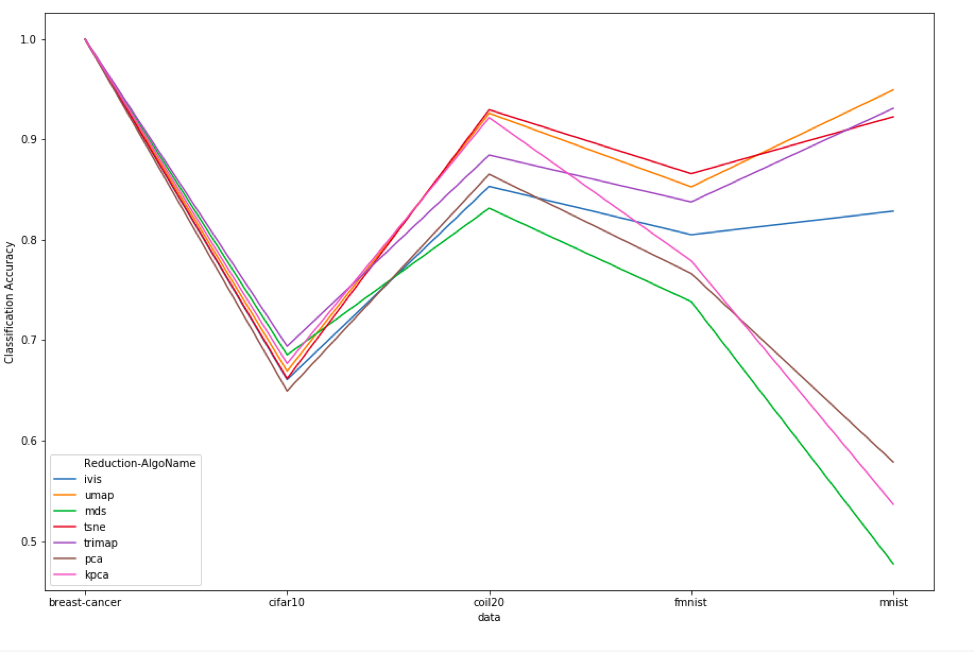
\includegraphics[width=0.94\linewidth]{class_acc.png}
	\label{fig:class_acc}
	\caption{Classification Accuracy}
\end{figure}
\\\textbf{Methodology}
\\Almost all the methods lead to almost 100\% accuracy in the breast-cancer dataset. One of the reasons, we think this happened is because the dataset size was very small which is why all the methods achieved near- perfect accuracy. COIL-20 dataset: We can see the methods achieving accuracy score in the range 80-94\%. MDS didn’t return great results and could only achieve around 80\% accuracy. t-SNE and UMAP were the best performers with both achieving around 93\% accuracy. For the CIFAR-10 dataset, we see an unusual trend with all the methods failing to achieve a score greater than 75\%. This might suggest some more in- depth analysis of the dataset, algorithms and data pre-processing. We also faced this anomaly for the MNIST dataset with PCA, kernel-PCA and MDS. MDS, probably, was the least expected to under-perform. It might have not been tuned correctly with the parameters, input pre-processed data due to which it achieved a score less than 50\%. In the F-MNIST dataset, the different methods achieved an accuracy score in the range of 75\% - 90\%. t-SNE and UMAP were expected to perform well given the quality of results and achieved a score close to 90\%. One thing to note was the performance of t-SNE and UMAP. We see that these two modern approaches out-perform most of the traditional methodologies. To get a better comparison between the two, we need to apply the two algorithms on larger datasets, use more quality features for dimensionality reduction, data pre-processing and study different parameters of both the algorithms that will help us rank the two.

\section{Mantel Test}
\\To establish how well a reduction algorithm, preserve data structure in low-dimensional space, a Euclidean distance based pairwise distance matrix was created for all of the seven datasets from their original embedding space as well as reduced embeddings. The level of correlation between the original distance matrix and the distance matrices in the embedding spaces was then assessed using the Mantel test. The Mantel Test is the Pearson’s product-moment correlation coefficient was used to quantitate concordance between original data and low-dimensional representations. We have used all the dataset that was used in the reduction technique which portrays the correct picture about good as well as bad examples of distance preservations.

\\The modified version of the Mantel test implementation takes two distance matrices (pairwise distances) and returns: correlation, the empirical p-value, and a standard score (z-score). We have chosen 10000 permutations and pearson correlation method to compute the correlations by default. For some of the datasets, due to lack of good computing resources, we reduced the number of permutations to 1000 (MNIST and Fashion-MNIST). Additionally, since many of the nearest neighbor algorithm suffer from poor indexing and slow retrieval, we have chosen the famous Annoy library from Spotify. Annoy creates large read-only file-based data structures that are mapped into memory so that many processes may share the same data.

\\Steps to complete Mantel Test:
\begin{itemize}
	\item Set the Annoy library to compute pairwise distances of input data.
	\item Compute the pairwise distance of original embedding space. For given n rows, it generated (n x n)
pairwise distance matrix.
	\item After reducing the embedding space to 2D, we calculate the pairwise distance of reduced dimension
space, we again get the same (n x n) pairwise matrix back.
    \item We pass these two obtained matrices to Mantel Test with 10000 permutations with upon performing
two tail statistical analysis; which returns a correlation value, an acceptable z-score (because of large permutations test, it always comes less than 0.05).
\end{itemize}

\begin{figure}[h!]
	\centering
	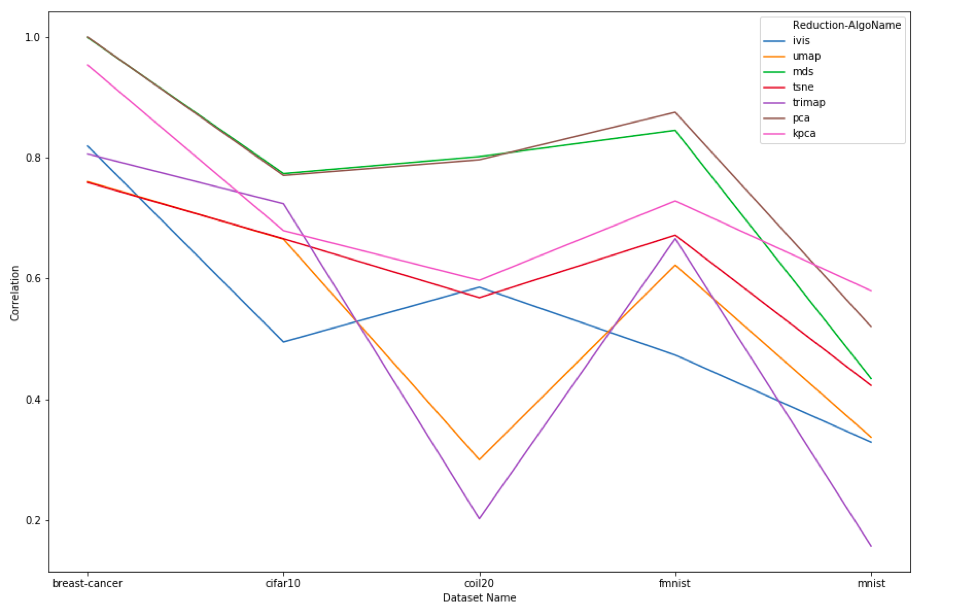
\includegraphics[width=0.94\linewidth]{mantel.png}
	\label{fig:mantel}
	\caption{Mantel Test Correlation Comparison}
\end{figure}
\vspace{5mm}
\\Key Takeaway Points from Mantel test:
\begin{itemize}
	\item It is interesting to see the low correlation in coil-20 and MNIST dataset, but at the same time it gives good accuracy with Fashion-MNIST dataset.
    \item MDS is able to keep the high correlation but many of SOP (self-organizing maps) like UMAP and tri- map which gave good accuracy scores but they fail to keep the distance preserved in lower dimension.
\end{itemize}

\addtolength{\textheight}{-12cm}   % This command serves to balance the column lengths
                                  % on the last page of the document manually. It shortens
                                  % the textheight of the last page by a suitable amount.
                                  % This command does not take effect until the next page
                                  % so it should come on the page before the last. Make
                                  % sure that you do not shorten the textheight too much.

%%%%%%%%%%%%%%%%%%%%%%%%%%%%%%%%%%%%%%%%%%%%%%%%%%%%%%%%%%%%%%%%%%%%%%%%%%%%%%%%


\begin{thebibliography}{99}

\bibitem{c1} G Corporación Unificada Nacional de Educación Superior (CUN). Problema General Proyectos Integradores. Circuitos de corriente alterna y laboratorio. $$ https://classroom.google.com/u/1/c/MTg2NzUyOTg4MTNa $$
\bibitem{c2} Factor de Potencia. Monografías. $$ http://www.monografias.com/trabajo14/factorpotencia/factorpotencia.shtml $$
\bibitem{c3} Factor de Potencia. Wikipedia – La Enciclopedia Libre. $$ http://www.es.wikipedia.org/wiki/Facotr_de_Potencia $$
[4]	¿Qué es el factor de potencia?
\bibitem{c4} ¿Qué es el factor de potencia? Potencia Aparente, Activa y Reactiva. https://youtu.be/5X4GRemc3pc
\bibitem{c5} Valor Medio y Valor Eficaz. $$ http://www.ifent.org/lecciones/cap08/cap08-05.asp $$
\bibitem{c6} Análisis de Circuitos eléctricos en estado estable y circuitos acoplados. $$ http://cimogsys.espoch.edu.ec/direccion_publicaciones/public/pdf/19an%C3%A1lisis%20circuitos%20en%20estado%20estable%20y%20circuitos%20acoplados_2.pdf 
$$

\end{thebibliography}




\end{document}

